\subsection{Calculus: change, accumulation, and several variables}
\label{math:calculus}

Calculus provides two complementary operations.
A derivative measures a local rate of change.
An integral measures accumulated change or total amount.
The fundamental theorem of calculus connects them.

\subsubsection{Derivatives as local rates of change}

For a function $y=f(t)$, the derivative is
\[
    \frac{\dd f}{\dd t}=\lim_{\Delta t\rightarrow0}\frac{f(t+\Delta t)-f(t)}{\Delta t}.
\]
The fraction before the limit is an average rate of change over a finite interval.
The derivative is the rate in the limit of an arbitrarily short interval.

Some basic derivative rules are
\[
    \frac{\dd}{\dd x}x^n=nx^{n-1}, \qquad \frac{\dd}{\dd x}e^{ax}=ae^{ax}, \qquad \frac{\dd}{\dd x}\ln x=\frac{1}{x}.
\]
The product and chain rules are
\[
    \frac{\dd}{\dd x}[f(x)g(x)]=f'(x)g(x)+f(x)g'(x),
\]
\[
    \frac{\dd}{\dd x}f(g(x))=f'(g(x))g'(x).
\]

\paragraph{Worked example: verify exponential relaxation}
Suppose a quantity relaxes toward a steady value $m_{\mathrm{ss}}$ over a timescale $\tau$:
\[
    m(t)=m_{\mathrm{ss}}+(m_0-m_{\mathrm{ss}})e^{-t/\tau}.
\]
Differentiating gives
\[
    \frac{\dd m}{\dd t}=-\frac{m_0-m_{\mathrm{ss}}}{\tau}e^{-t/\tau}.
\]
The displacement from steady state is $m(t)-m_{\mathrm{ss}}=(m_0-m_{\mathrm{ss}})e^{-t/\tau}$.
Therefore
\[
    \frac{\dd m}{\dd t}=-\frac{m-m_{\mathrm{ss}}}{\tau},
\]
which says directly that the system moves toward steady state at a rate proportional to its remaining displacement.

\subsubsection{Partial derivatives}

A function of several variables can change in several independent directions.
For $P=P(x,t)$, $\partial P/\partial t$ measures change with time while holding position fixed, whereas $\partial P/\partial x$ measures spatial change at fixed time.
The second spatial derivative $\partial^2P/\partial x^2$ measures how the slope changes with position.
At a smooth local maximum it is typically negative, and at a smooth local minimum it is typically positive.
This explains qualitatively why the diffusion equation lowers peaks and fills valleys.

\subsubsection{Integrals as accumulated quantities}

The definite integral $\int_a^b f(x)\,\dd x$ is the signed area accumulated under $f$ between $a$ and $b$.
If $F'(x)=f(x)$, the fundamental theorem of calculus gives
\[
    \int_a^b f(x)\,\dd x=F(b)-F(a).
\]

\paragraph{Worked example: normalize an exponential density}
For $p(t)=\lambda e^{-\lambda t}$ with $t\geq0$ and $\lambda>0$,
\[
    \int_0^{\infty}p(t)\,\dd t=\left[-e^{-\lambda t}\right]_{0}^{\infty}=1.
\]

\subsubsection{The continuity equation}

Let $\rho(x,t)$ be an amount per unit length and $J(x,t)$ the amount crossing a point per unit time.
Conservation implies
\[
    \frac{\partial\rho}{\partial t}=-\frac{\partial J}{\partial x}.
\]
Integrating over an interval gives
\[
    \frac{\dd}{\dd t}\int_a^b\rho(x,t)\,\dd x=J(a,t)-J(b,t).
\]


\subsection{Taylor expansions and controlled approximations}
\label{math:taylor}

A Taylor expansion replaces a function near a chosen point by a polynomial whose value and derivatives match those of the function.
For expansion around $x_0$,
\[
    f(x)=f(x_0)+f'(x_0)(x-x_0)+\frac{f''(x_0)}{2!}(x-x_0)^2+\cdots.
\]
The notation $\mathcal{O}((x-x_0)^2)$ denotes an omitted error of second order or smaller as $x\rightarrow x_0$.

\begin{figure}[ht]
    \centering
    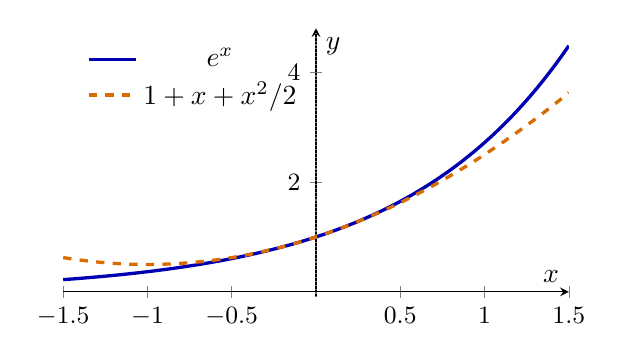
\begin{tikzpicture}
        \begin{axis}[
            width=0.66\textwidth,
            height=5.0cm,
            axis lines=middle,
            xlabel={$x$},
            ylabel={$y$},
            xmin=-1.5,
            xmax=1.5,
            ymin=-0.1,
            ymax=4.8,
            samples=120,
            legend style={draw=none,fill=none,at={(0.03,0.97)},anchor=north west},
            tick label style={font=\small}
        ]
            \addplot[very thick,blue!70!black,domain=-1.5:1.5] {exp(x)};
            \addlegendentry{$e^x$}
            \addplot[very thick,dashed,orange!85!black,domain=-1.5:1.5] {1+x+x^2/2};
            \addlegendentry{$1+x+x^2/2$}
            \addplot[thin,densely dotted,black!55] coordinates {(0,-0.1) (0,4.8)};
        \end{axis}
    \end{tikzpicture}
    \caption{The quadratic Taylor approximation to $e^x$ agrees with the function near the expansion point and gradually departs from it farther away}
    \label{fig:taylor-approximation}
\end{figure}

Common expansions are
\[
    e^x=1+x+\frac{x^2}{2!}+\cdots, \qquad \sin x=x-\frac{x^3}{3!}+\cdots,
\]
\[
    \cos x=1-\frac{x^2}{2!}+\cdots, \qquad \ln(1+x)=x-\frac{x^2}{2}+\cdots.
\]

\paragraph{Worked example: the continuum limit}
Expanding $P(x+a,t)$ and $P(x-a,t)$ around $x$ and adding gives
\[
    P(x+a,t)+P(x-a,t)-2P(x,t)=a^2\frac{\partial^2P}{\partial x^2}+\mathcal{O}(a^4).
\]
Odd powers cancel because the walk is symmetric.

\paragraph{Common mistakes}
\begin{itemize}
    \item State the small quantity, such as $a/L\ll1$.
    \item A Taylor approximation is local, not automatically global.
    \item Smoothness supports finite expansions with remainders, but an infinite Taylor series need not equal every smooth function.
\end{itemize}


\subsection{Linear interpolation}
\label{math:interpolation}

For known points $(x_1,y_1)$ and $(x_2,y_2)$, linear interpolation gives
\[
    y(x)=y_1+\frac{y_2-y_1}{x_2-x_1}(x-x_1).
\]

\begin{figure}[ht]
    \centering
    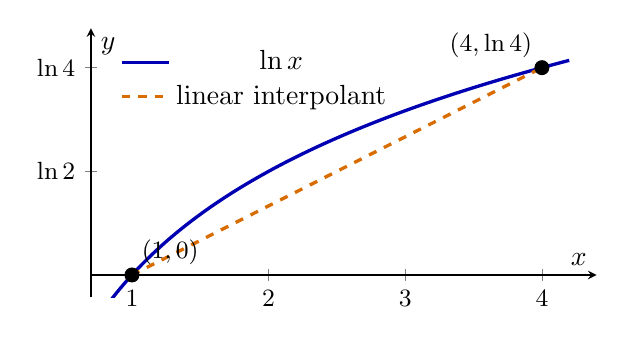
\begin{tikzpicture}
        \begin{axis}[
            width=0.66\textwidth,
            height=5.0cm,
            axis lines=middle,
            xlabel={$x$},
            ylabel={$y$},
            xmin=0.7,
            xmax=4.4,
            ymin=-0.15,
            ymax=1.65,
            xtick={1,2,3,4},
            ytick={0,0.693,1.386},
            yticklabels={$0$,$\ln2$,$\ln4$},
            legend style={draw=none,fill=none,at={(0.04,0.96)},anchor=north west},
            tick label style={font=\small},
            samples=120
        ]
            \addplot[very thick,blue!70!black,domain=0.8:4.2] {ln(x)};
            \addlegendentry{$\ln x$}
            \addplot[very thick,dashed,orange!85!black,domain=1:4] {(ln(4)/3)*(x-1)};
            \addlegendentry{linear interpolant}
            \addplot[only marks,mark=*,mark size=2.5pt,black] coordinates {(1,0) (4,1.386294)};
            \node[anchor=south west,font=\small] at (axis cs:1,0) {$(1,0)$};
            \node[anchor=south east,font=\small] at (axis cs:4,1.386294) {$(4,\ln4)$};
        \end{axis}
    \end{tikzpicture}
    \caption{Linear interpolation of the concave function $\ln x$ between two known points. The interpolating line lies below the function between the endpoints}
    \label{fig:linear-interpolation}
\end{figure}

\paragraph{Worked example}
For $y=\ln x$, use the known points $(1,0)$ and $(4,\ln4)$.
The interpolating line is
\[
    y_{\mathrm{lin}}(x)=\frac{\ln4}{3}(x-1).
\]
At $x=2$, it gives $y_{\mathrm{lin}}(2)=\ln4/3\approx0.462$, whereas $\ln2\approx0.693$.
Because $\ln x$ bends downward, its secant line lies below the curve, so this interpolation underestimates the function between the endpoints.
